\label{chap:implementation}
This chapter, together with Chapter~\ref{chap:design}, answers Research Question~2:

\begin{quote}
\textit{How can we design and implement a hybrid interface that combines graph-based visualisation with table-based planning to help students plan their studies and understand curriculum structure and course dependencies, based on those requirements?}
\end{quote}

Chapter~\ref{chap:design} answers the design half; this chapter describes the tool that realises it. The tool is a contribution of this thesis, but it is not its subject: it is the instrument through which the design is evaluated. The chapter therefore records the architecture and the components that matter for reproducing the tool and for trusting the evaluation, and refers back to Chapter~\ref{chap:design} for the interface behaviour it realises rather than restating it. Alongside the study planner, a small questionnaire application was built to conduct the evaluation sessions; it is described briefly in Section~\ref{sec:impl-userstudy}.

\section{System Overview}
\label{sec:impl-overview}

The study planner is a single-page web client backed by a stateless HTTP service and a relational database (Figure~\ref{fig:impl-architecture}). The client is a React\footnote{\url{https://react.dev}, version~18.3.1.} application built with Vite\footnote{\url{https://vite.dev}, version~5.4.20.}, and renders both the graph and the Table View on a single interactive canvas provided by React~Flow\footnote{\url{https://reactflow.dev}, version~11.11.4.}. The service is written in Python with FastAPI\footnote{\url{https://fastapi.tiangolo.com}.} and encapsulates catalogue access, plan persistence, curriculum-compliance checking, and recommendation. Data is stored in PostgreSQL\footnote{\url{https://www.postgresql.org}, version~16.}. This separation places presentation on the client, logic on the server, and data in the database, which is the arrangement the requirements already imply, with interface features (for example the graph-to-table workflow, Feature~\ref{feat:004}) kept distinct from the logic-heavy compliance (Feature~\ref{feat:003}) and recommendation (Feature~\ref{feat:007}) features.

In deployment, the client and the questionnaire application are served on Vercel\footnote{\url{https://vercel.com}.}, the FastAPI service runs on Render\footnote{\url{https://render.com}.}, and the database is a managed PostgreSQL instance on Neon\footnote{\url{https://neon.tech}.}; the \texttt{docker-compose} configuration in the repository provides an equivalent stack for local development. Client and service exchange JSON over two paths, plan persistence and read-only consultation, and the service's own structure is the subject of Figure~\ref{fig:impl-backend-components}.
\begin{figure}[htbp]
\centering
\begin{tikzpicture}[font=\small,
  tier/.style={draw, line width=1pt, rounded corners=3pt, minimum width=3.6cm, minimum height=30mm, fill=white},
  tab/.style={draw, line width=1pt, fill=white, font=\bfseries\small, inner sep=3pt, rounded corners=1.5pt},
  row/.style={font=\small, align=left},
  dep/.style={font=\scriptsize\itshape, text=black},
  flow/.style={-{Latex[length=3mm]}, line width=1.2pt, draw=black},
  flowalt/.style={-{Latex[length=3mm]}, line width=1.2pt, draw=black, dash pattern=on 4pt off 2.5pt}]
  \node[tier] (client) {};
  \node[tier, right=17mm of client] (api) {};
  \node[tier, right=17mm of api] (db) {};
  \node[tab, anchor=south west] at ($(client.north west)+(2mm,-1mm)$) {Browser client};
  \node[tab, anchor=south west] at ($(api.north west)+(2mm,-1mm)$) {API service};
  \node[tab, anchor=south west] at ($(db.north west)+(2mm,-1mm)$) {Database};
  \node[row, below=4mm of client.north] (c1) {
\includegraphics[height=4mm]{pictures/icons/react.pdf}\ \ React};
  \node[row, below=2.3mm of c1.south, anchor=north] (c2) {\phantom{
\includegraphics[height=4mm]{pictures/icons/react.pdf}}\ \ React~Flow};
  \node[row, below=2.3mm of c2.south, anchor=north] (c3) {
\includegraphics[height=4mm]{pictures/icons/vite.pdf}\ \ Vite};
  \node[row, below=7mm of api.north] (a1) {
\includegraphics[height=4mm]{pictures/icons/fastapi.pdf}\ \ FastAPI};
  \node[row, below=7mm of db.north] (d1) {
\includegraphics[height=4mm]{pictures/icons/postgresql.pdf}\ \ PostgreSQL};
  \coordinate (depc) at ($(client.south)+(0,-4.8mm)$);
  \coordinate (depa) at ($(api.south)+(0,-4.8mm)$);
  \coordinate (depd) at ($(db.south)+(0,-4.8mm)$);
  \node[dep] at (depc) {
\includegraphics[height=3.4mm]{pictures/icons/vercel.pdf}\ \ on Vercel};
  \node[dep] at (depa) {
\includegraphics[height=3.4mm]{pictures/icons/render.pdf}\ \ on Render};
  \node[dep] at (depd) {
\includegraphics[height=3.4mm]{pictures/icons/neon.pdf}\ \ on Neon};
  \draw[flow] ($(client.east)+(0,4mm)$) -- node[above, font=\scriptsize]{persist} ($(api.west)+(0,4mm)$);
  \draw[flowalt] ($(client.east)+(0,-4mm)$) -- node[below, font=\scriptsize]{consult} ($(api.west)+(0,-4mm)$);
  \draw[flow] (api) -- node[above, font=\small]{SQL} (db);
\end{tikzpicture}
\caption{The three tiers of the study planner, the main technology in each, and where each is hosted. Client and service exchange JSON over HTTPS; only the service touches the database.}
\label{fig:impl-architecture}
\end{figure}

\section{Frontend}
\label{sec:impl-frontend}

The client realises the interface designed in Chapter~\ref{chap:design} and is the larger of the two applications. It is organised in three layers (Figure~\ref{fig:impl-frontend-layers}): the feature modules use the domain layer and the API client, and the domain layer uses neither. What follows takes them in the order the figure draws them, from the top down.

\begin{figure}[htbp]
\centering
\begin{tikzpicture}[font=\small,
  layer/.style={draw, line width=1pt, rounded corners=3pt, fill=white, align=left,
                inner sep=2.8mm, text width=10.2cm},
  tab/.style={draw, line width=1pt, fill=white, font=\bfseries\small, inner sep=2pt,
              rounded corners=1.5pt},
  a/.style={-{Latex[length=2.6mm]}, line width=1.1pt, draw=black},
  lb/.style={font=\scriptsize, inner sep=1.2pt}]
  \node[layer, minimum height=15mm] (features) {\ \\[1mm]
    \small profile, catalogue, Dashboard, recommendations, onboarding tour,\\
    \small prebuilt plans, compliance feedback, planning canvas \\[1.2mm]
    \small each owns its state, its effects and the components that render it};
  \node[tab, anchor=south west] at ($(features.north west)+(3mm,-1.2mm)$) {Feature modules};

  \node[layer, below=9mm of features, minimum height=13mm] (domain) {\ \\[1mm]
    \small plan reducer, term and lane rules, lane geometry, graph filters,\\
    \small prebuilt-plan builders \\[0.8mm]
    \small no framework, no browser, no network};
  \node[tab, anchor=south west] at ($(domain.north west)+(3mm,-1.2mm)$) {Domain};

  \node[layer, below=9mm of domain, minimum height=7mm] (client) {\ \\[0.5mm]
    \small one module for every request the client makes};
  \node[tab, anchor=south west] at ($(client.north west)+(3mm,-1.2mm)$) {API client};

  \draw[a] (features) -- node[lb, right] {depends on} (domain);
  \draw[a, rounded corners=2pt] (features.west) -- ++(-1.15,0)
    |- node[lb, pos=0.45, anchor=east, xshift=-1.2mm] {depends on} (client.west);
\end{tikzpicture}
\caption{The client's three layers. A feature module may use the domain layer and the API client; the domain layer uses neither and needs no browser to run.}
\label{fig:impl-frontend-layers}
\end{figure}

\paragraph{Feature Modules}
At the top, the client is divided by feature rather than by technical kind. Each of the profile, the catalogue, the Dashboard, the Recommendation Panel, the onboarding tour, the prebuilt plans, the compliance feedback and the planning canvas is a module holding its own state, its own effects and the components that render it; the screen is assembled from them. A module may depend on the layer beneath it and on no other module, so a change to one feature cannot reach another except through the plan they share.

\paragraph{The Domain Layer}
The domain layer holds the rules for terms and lanes, which decide the season a lane carries and whether a course may be offered in it; the lane geometry that turns a drop position into a semester; the graph's filter matching, which keeps a matched course's whole ancestry on screen; the builders behind the prebuilt plans; and, at its centre, the plan and the reducer that changes it. All of it lives there on the terms the figure states: it imports no framework, so neither React nor React Flow; touches no browser object; and makes no request. Each part is therefore exercised by calling it.

That plan is what a student builds and what everything else in the tool reads: the courses filed under each semester, the codes marked done and the codes parked, the notes, hour estimates and grades on individual courses, the note on each semester, the chosen focus area, the workload limits, and what the graph remembers between visits, its filters, its collapsed nodes and the positions nodes have been dragged to. One such plan is held for each programme a student has opened, and the account holds the set of them. The Graph View and the Table View are two projections of that plan: switching view changes how the plan is drawn, never which plan is described, and persistence, the Dashboard, compliance feedback and recommendations are all derived from the same model.

The reducer is a pure function from the current plan and a described change to the next plan; marking a course complete, applying a prebuilt plan, switching programme, choosing a focus area and clearing the plan are dispatched to it as discrete changes, each exercisable by calling it rather than by rendering the interface around it.

Placing, moving and parking a course in the Table View are handled differently. The board's node array is built from the plan when a programme is opened, and on every commit the array is written back whole rather than as a single described move, because one interaction rarely moves one card: collision spacing, module group clearance and the relocation of courses stranded by a change of start term shift others at the same time, and writing the array back captures all of them at once. The canvas is therefore an input to the plan and not only a rendering of it.

The Graph View does not take part in this. Its node positions encode curriculum depth and subject band, so dragging there changes a remembered offset and nothing else. Adding a course from the graph does reach the plan through the same array, but its lane is named by the \gterm{semester-picker}{Semester Picker} (Section~\ref{sec:semester-picker}) rather than read from where a card was dropped.

\paragraph{The API Client}
A single foundational network module encapsulates all client-service communication via fourteen explicit request functions (handling authentication, catalogue data, plan persistence, profile settings, compliance, and recommendations). By restricting all network connections exclusively to this module, the architecture enforces strict layering. Additionally, the module localizes all transport-level configurations (such as service endpoints, bearer tokens, and payload structures), ensuring the upper application layers remain entirely agnostic to the network implementation.

\subsection{How an Edit Travels}
State mutations follow a strict unidirectional data flow (Figure~\ref{fig:impl-edit-flow}). While standard UI inputs (such as the Semester Picker or text fields) dispatch discrete actions, Table View drags introduce an architectural exception. As established, drag interactions return the updated node array, mapping horizontal coordinates to planned semesters. Consequently, this is the single instance where the canvas acts as a direct state input rather than a pure rendering layer.

Once an action or drag is processed by the plan reducer, the resulting state update triggers two independent execution paths. Synchronously, pure layout functions recalculate affected graph columns or table lanes to trigger a view re-render. Asynchronously, the updated plan is persisted to the backend, while the compliance and recommendation endpoints are queried to update the Dashboard and transient feedback banners. Network persistence is debounced by 500 milliseconds to prevent excessive writes during exploratory interactions. While API consultations are not debounced, they mitigate race conditions via request identifiers: stale responses arriving after a subsequent edit are explicitly discarded rather than applied out of order.

Finally, the course lifecycle (Section~\ref{sec:lifecycle}) requires no dedicated state-machine controller. Course states are handled declaratively within the plan, transitions are managed entirely by the reducer, and valid action buttons are derived dynamically at render time. Graph visibility is computed similarly: a self-contained module evaluates courses against active filters and preserves every ancestor of a match, so a matched course is never hidden because its module or exam subject was filtered out (Section~\ref{sec:graph-spatial}).


\begin{figure}[htbp]
\centering
\begin{tikzpicture}[font=\small, node distance=0mm,
  box/.style={draw, line width=1pt, rounded corners=3pt, fill=white, align=center,
              inner sep=2.6mm, text width=4.6cm, minimum height=11mm},
  hub/.style={box, text width=5.4cm},
  tab/.style={draw, solid, line width=1pt, fill=white, font=\bfseries\scriptsize,
              inner sep=2pt, rounded corners=1.5pt},
  a/.style={-{Latex[length=2.8mm]}, line width=1.2pt, draw=black},
  ad/.style={a, dash pattern=on 4pt off 2.5pt},
  lb/.style={font=\scriptsize\itshape, inner sep=1.4pt, fill=white}]
  \node[hub] (act) {\textbf{Drag or button action}};
  \node[hub, below=8mm of act] (model) {\textbf{Plan reducer}\\[0.6mm] \small produces the next plan};
  \coordinate (fork) at ($(model.south)+(0,-9mm)$);

  \node[box, below left=19mm and -1.2cm of model] (reflow)
        {\textbf{Pure layout functions}\\[0.6mm] \small reflow lanes and graph columns};
  \node[box, below right=19mm and -1.2cm of model] (persist)
        {\textbf{Persist and consult}\\[0.6mm] \small debounced save, immediate checks};
  \node[box, below=8mm of reflow] (render) {\textbf{Active view}\\[0.6mm] \small re-renders};
  \node[box] (dash) at (render -| persist)
        {\textbf{Dashboard and banners}\\[0.6mm] \small update};

  \draw[a] (act) -- (model);
  \draw[line width=1.2pt] (model) -- (fork);
  \draw[a] (fork) -| node[tab, pos=0.28, above=1.4mm] {immediate} (reflow.north);
  \draw[ad] (fork) -| node[tab, pos=0.28, above=1.4mm] {off the render path} (persist.north);
  \draw[a] (reflow) -- (render);
  \draw[ad] (persist) -- (dash);
\end{tikzpicture}
\caption{Edits follow one direction. A transition produces the next plan, from which an immediate re-render follows and, off the render path, a debounced save and an immediate consultation.}
\label{fig:impl-edit-flow}
\end{figure}


\subsection{What a Student Sees}
The layers above describe how the code is arranged. What they present is the three-panel shell of Section~\ref{sec:three-panels}: the catalogue, its filters and the Recommendation Panel on the left, the Graph View or the Table View in the centre, and the Dashboard on the right, reached through a gate that handles sign-in and, on first entry, collects the programme and start term (Section~\ref{sec:onboarding}). Figure~\ref{fig:three-panels} draws the arrangement using the example of the Graph View, and the figures that follow show the individual components: the shell as a student meets it (Figure~\ref{fig:impl-shot-shell}), then the Graph (Figure~\ref{fig:impl-shot-graph}), the Table (Figure~\ref{fig:impl-shot-table}), the two side panels (Figure~\ref{fig:impl-shot-recs}) and the catalogue sidebar beside the profile dialogue (Figure~\ref{fig:impl-shot-catalogue-profile}).



\begin{figure}[htbp]
\centering
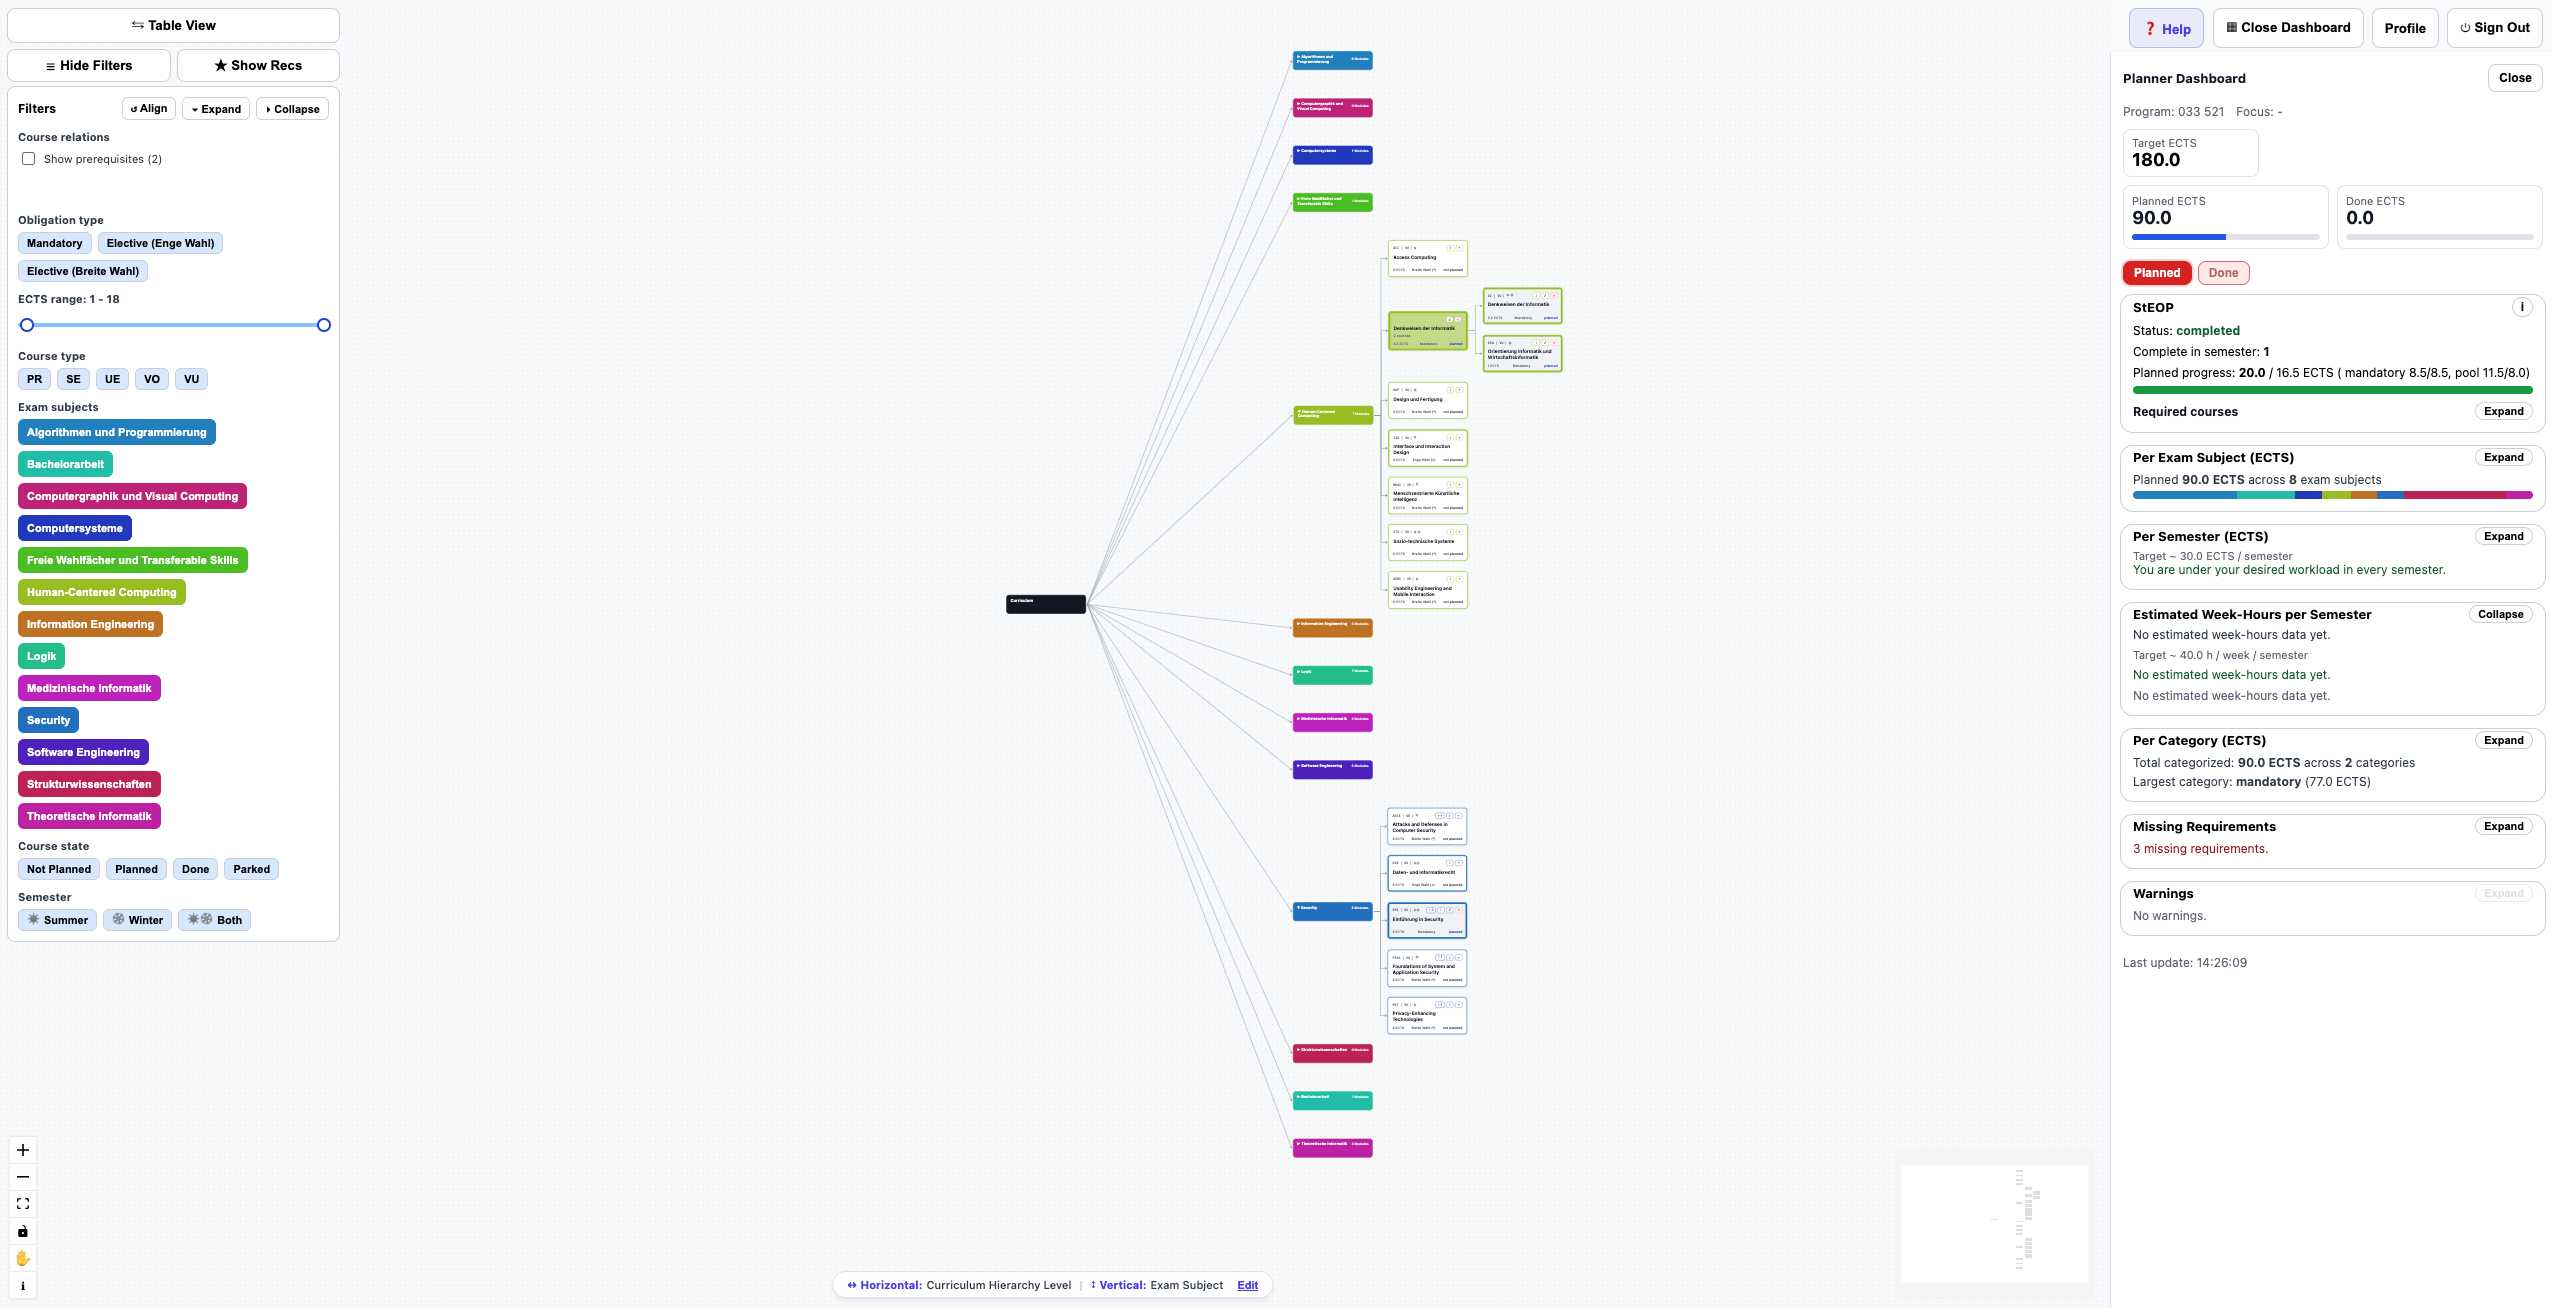
\includegraphics[width=\textwidth]{pictures/Full_graph_view_Screenshot.png}
\caption{The whole tool in the Graph View: the catalogue and its filters on the left, the curriculum in the centre, and the Dashboard on the right.}
\label{fig:impl-shot-shell}
\end{figure}

\begin{figure}[htbp]
\centering
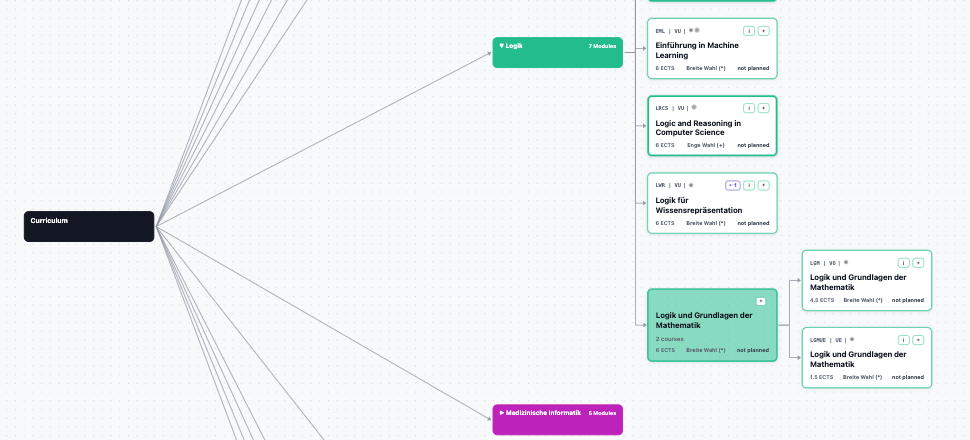
\includegraphics[width=\textwidth]{pictures/Graph_view_crop.png}
\caption{The Graph View, with all four levels in one frame: the programme root, an exam subject, its courses, and a module holding two courses drawn as its own node.}
\label{fig:impl-shot-graph}
\end{figure}

\begin{figure}[htbp]
\centering
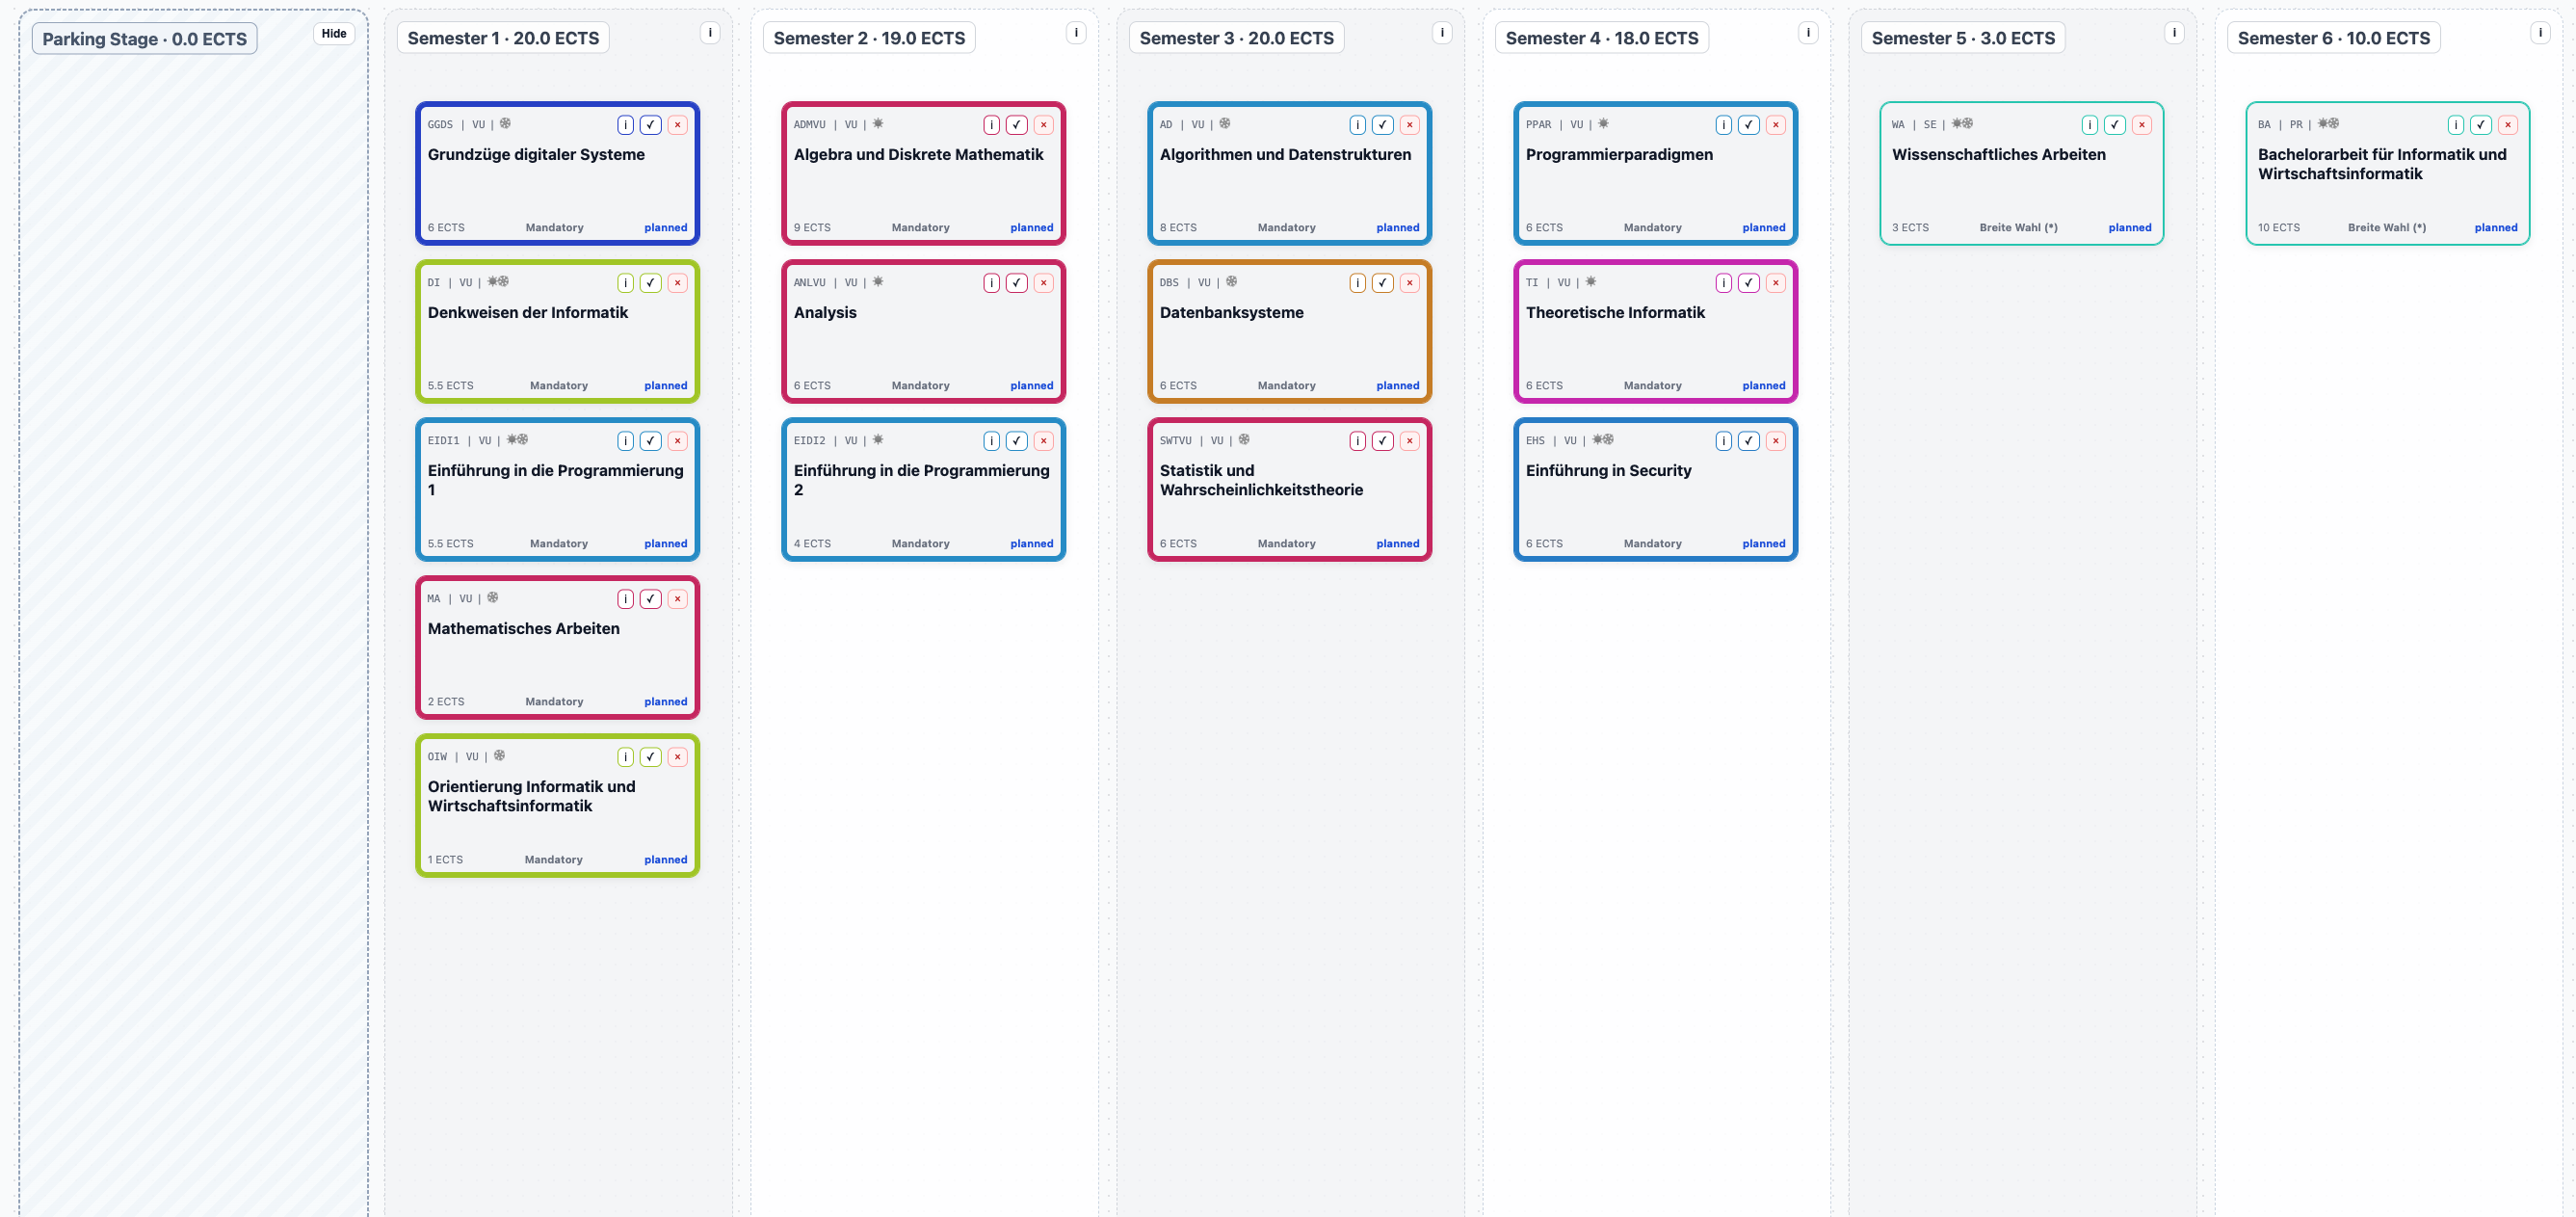
\includegraphics[width=\textwidth]{pictures/Table_Screenshot.png}
\caption{The Table View: the same plan arranged into semester lanes with their credit totals, and a Parking Stage on the left holding courses a student has shortlisted but not yet scheduled.}
\label{fig:impl-shot-table}
\end{figure}

\begin{figure}[htbp]
\centering
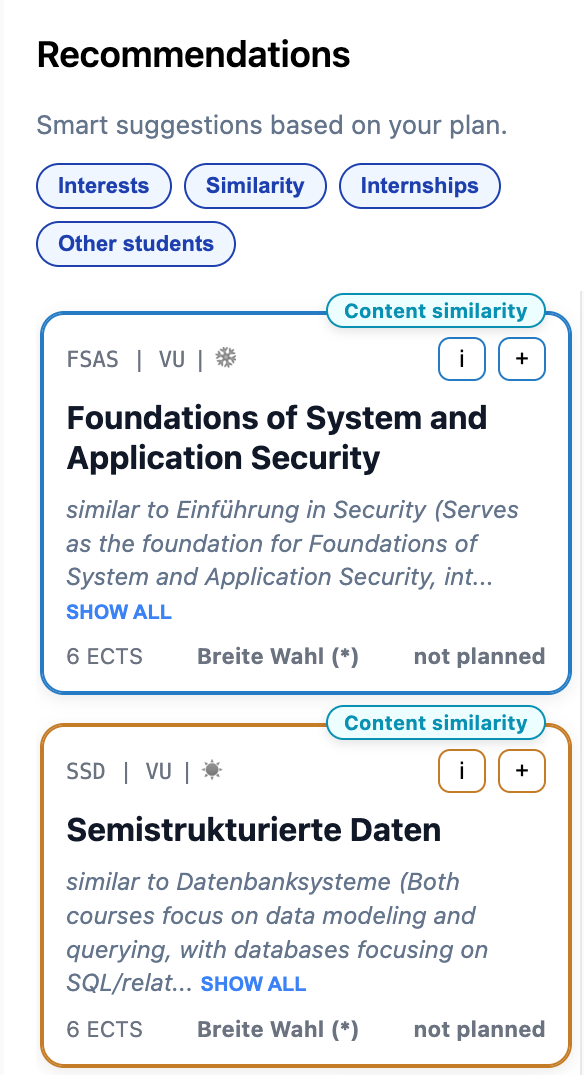
\includegraphics[height=8.6cm]{pictures/Recommendation_panel_crop.png}\hspace{6mm}%
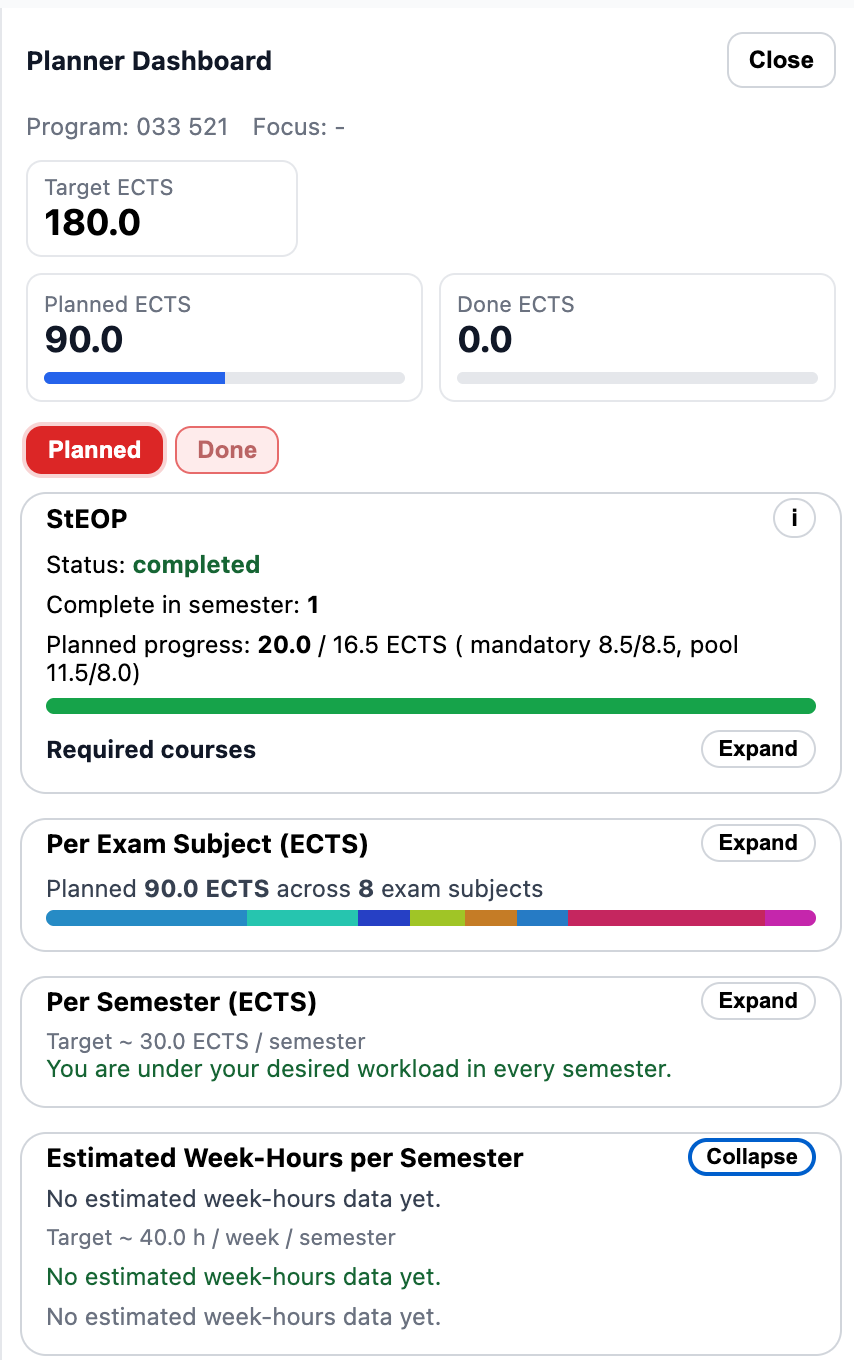
\includegraphics[height=8.6cm]{pictures/Dashboard_crop.png}
\caption{The two side panels: the Recommendation Panel, whose cards name the family that produced them, and the Dashboard, where the Compliance Engine's answer becomes visible. Both continue below the crop.}
\label{fig:impl-shot-recs}
\end{figure}

\begin{figure}[htbp]
\centering

\includegraphics[height=8.4cm]{pictures/Sidebar_Screenshot.png}\hspace{6mm}%
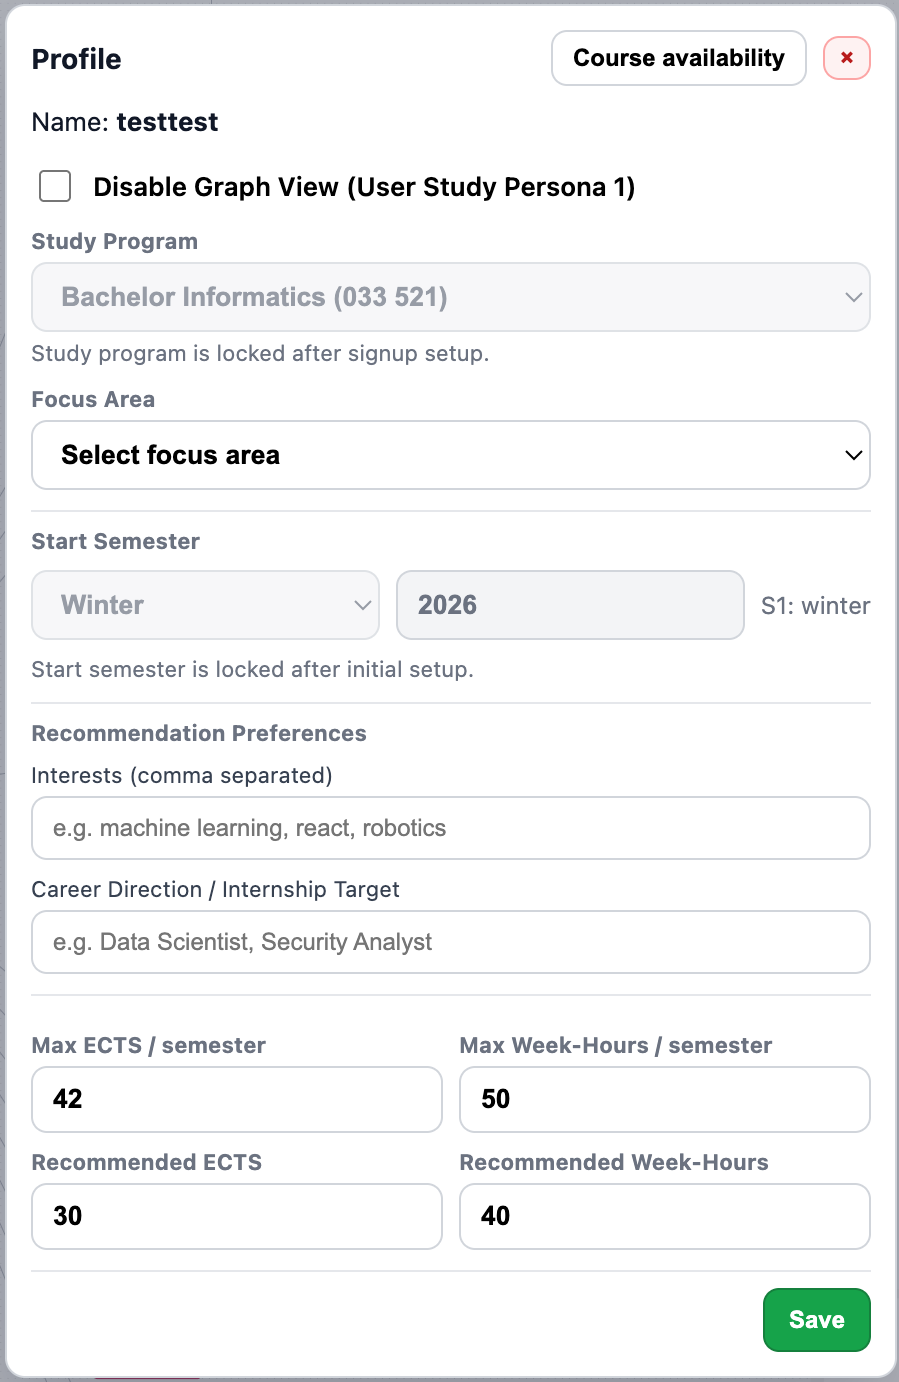
\includegraphics[height=8.4cm]{pictures/Profile__Screenshot.png}
\caption{The catalogue sidebar, grouped by exam subject with collapsible modules, and the profile dialogue holding the focus area, the recommendation preferences and the workload limits.}
\label{fig:impl-shot-catalogue-profile}
\end{figure}




\section{Backend}
\label{sec:impl-backend}

The backend service provides three functions: persistence of the study plan, curriculum compliance evaluation, and course recommendation. It is a FastAPI application structured in four layers with a strictly downward dependency direction (Figure~\ref{fig:impl-backend-components}). Request handlers validate input, invoke exactly one use case, and serialise the response; they contain no domain logic and no SQL. Use cases orchestrate domain operations and define the transaction boundary; eight service modules cover authentication and sessions, catalogue retrieval, prerequisite relations, plan persistence, profile settings, compliance evaluation, recommendation, and the capture of study results, which are stored as one file per questionnaire submission (Section~\ref{sec:impl-userstudy}). The domain layer comprises two packages, compliance and recommendation, described in Sections~\ref{sec:impl-compliance} and~\ref{sec:impl-recommender}. Repositories encapsulate all SQL statements.

Use cases access storage exclusively through a unit-of-work abstraction: an object that provides every repository bound to a single database connection. A use case therefore neither acquires connections nor references concrete repository classes. Two properties follow: a use case can be tested against a substitute unit of work without a database, and the set of statements that must commit atomically is declared in the use case rather than determined by repository execution order. Domain failures are raised as typed exceptions named for their cause, for instance \texttt{ProgrammeLocked}, \texttt{StartTermLocked} and \texttt{SetupIncomplete}; a single mapping table translates exception types to HTTP status codes and is the only component of the service aware of HTTP semantics. Authentication resolves the user from a session token supplied either as a cookie or as a bearer token, so that the deployed and the local client authenticate against an unchanged service. Persistence uses a shared PostgreSQL connection pool with parameterised SQL; no object-relational mapper is employed.

\begin{figure}[htbp]
\centering
\begin{tikzpicture}[font=\small,
  card/.style={draw, line width=1pt, rounded corners=3pt, fill=white, align=left, inner sep=2.5mm},
  wide/.style={card, text width=9.7cm},
  half/.style={card, text width=3.4cm, minimum height=13mm},
  a/.style={-{Latex[length=2.6mm]}, line width=1.1pt, draw=black},
  lb/.style={font=\scriptsize, inner sep=1.4pt, fill=white}]
  \node[wide] (api) {\textbf{Request handlers} \\[0.8mm] \small validate, call one use case, shape the reply};
  \node[wide, below=7mm of api] (svc) {\textbf{Use cases} \\[0.8mm] \small auth, catalogue, plan state, profile,\\ \small compliance, recommendation};
  \node[half, anchor=north west] (dom) at ($(svc.south west)+(0,-11mm)$) {\textbf{Compliance} \\[0.8mm] \small one rule set per programme, over the curriculum as data};
  \node[half, anchor=north east] (rec) at ($(svc.south east)+(0,-11mm)$) {\textbf{Recommendation} \\[0.8mm] \small six channels behind one protocol};
  \node[wide, anchor=north] (repo) at ($(dom.south)!0.5!(rec.south)+(0,-11mm)$) {\textbf{Repositories} \\[0.8mm] \small every SQL statement, bound to one connection by a unit of work};
  \coordinate (fork) at ($(svc.south)+(0,-5.5mm)$);
  \draw[a] (api) -- (svc);
  \draw[line width=1.1pt] (svc) -- (fork);
  \draw[a] (fork) -| (dom.north);
  \draw[a] (fork) -| (rec.north);
  \draw[a, rounded corners=2pt] (svc.west) -- ++(-11mm,0)
    |- node[lb, pos=0.45, anchor=east, xshift=-1.2mm] {reaches storage through} (repo.west);
  \draw[a] (rec.west) -- node[lb] {re-checks} (dom.east);
\end{tikzpicture}
\caption{Backend layers, under the same one-way dependency rule as the client: handlers hold no rules and no SQL, use cases own the transaction boundary, and the recommender re-checks every suggestion.}
\label{fig:impl-backend-components}
\end{figure}

\subsection{Curriculum Compliance Engine}
\label{sec:impl-compliance}

The Compliance Engine implements Feature~\ref{feat:003} and Feature~\ref{feat:005}. All rules are derived from the published curricula of the two supported programmes, the Bachelor programme in Computer Science and the Master programme in Software Engineering\footnote{\url{https://informatics.tuwien.ac.at/bachelor/curriculum-ue033521.pdf}, \url{https://informatics.tuwien.ac.at/master/curriculum-ue066937.pdf}; the versions in force during this work were used.}; no rule has another source.

Curriculum content is separated from evaluation logic. Each programme's regulations are encoded as a JSON document in \texttt{app/curriculum/}, comprising modules and credit weights, the course-to-module mapping, the introductory-phase course sets, focus areas with their aliases, prerequisite pairs, and numeric thresholds (nine constants for the Bachelor programme, five for the Master). The two documents do not share a schema: the Master document contains no course-to-module mapping, focus areas or introductory phase, as its curriculum defines none. Each checker loads its document once at construction; a curriculum revision therefore modifies data, not code.

Evaluation is performed by one rule set per programme, selected by programme code. The two rule sets share only the request format, the result schema, the entry point and the interpretation of credit limits. The Bachelor rule set enforces the introductory phase (\gterm{steop}{StEOP}); the Master rule set enforces its prerequisite pairs and emits a warning when the electives of an exam subject precede its core modules; neither rule has a counterpart in the other curriculum. No common base class was introduced, since the shared logic is smaller than the abstraction required to express it; whether a common core emerges with a third programme is left to future work.

For a submitted plan, the engine computes credit totals per semester and per exam subject and evaluates them against the curriculum: semester load against the absolute ceiling and the recommended load, module completeness and exam-subject minima, prerequisite and sequencing rules, and the total credit requirement. Findings are classified in two tiers, so that the interface guides rather than blocks (Section~\ref{sec:overall-scope}). An error, for instance a semester exceeding its ceiling or a violated hard prerequisite, rejects the triggering change, which the client reverts; a warning, for instance a semester exceeding its recommended load or an elective scheduled before its subject's core modules, is advisory. The result additionally carries the statistics rendered by the Dashboard, so that interface and rule engine derive from a single computation. The recommendation engine invokes the same checker to validate every candidate suggestion (Section~\ref{sec:impl-recommender}).

\subsection{Recommendation Support}
\label{sec:impl-recommender}

The recommendation component implements the recommendation workflow of the design (Feature~\ref{feat:007}, Feature~\ref{feat:012}). It is not a contribution to recommender-systems research, and the accuracy of its methods is excluded from scope by OOS5. It combines established techniques: content-based matching against stated interests and curated course similarities, sequence relations of the kind proposed by sequence-based course recommenders~\cite{wong_sequence_2018}, and a collaborative-filtering component modelled on elective recommendation~\cite{bhumichitr_recommender_2017}. The collaborative component operates on a synthetically generated cohort of prior-student plans rather than on real interaction data; it therefore reproduces the workflow of a data-driven recommender, not its performance.

Six channels implement a common protocol consisting of a name and a single scoring method that returns a score and an evidence string for a candidate course. The interest channel weights an explicit topic match above a description match and a partial keyword overlap below both, normalised by the number of stated interests. The similarity channel performs no inference; it reads curated course-to-course links stored in the catalogue, each carrying the justification presented as evidence (Figure~\ref{fig:impl-shot-recs}). The sequence channel reads the orderings the curricula define between named courses. The follow-on channel scores a candidate by the proportion of cohort members who took it after a course the student has completed and suppresses proportions below a majority; the peer channel scores it by the proportion among the cohort members whose plans most overlap the student's, and reverts to overall popularity, flagged as such, for an empty plan. The internship channel matches the stated career direction against course skills and descriptions. The engine queries the channels in a fixed order, retains one record per course, sorts by score, and validates each of the top hundred records against the Compliance Engine by trial placement, discarding any record that would introduce an error or a warning absent from the baseline evaluation; at most fifteen records are returned. Since scores are assigned per channel, a channel with a fixed high score, such as curated similarity, dominates the top of the list.

All six families were active during the sessions reported in Chapter~\ref{chap:evaluation}. Four depend on student-supplied data or on the synthetic cohort and return no results without input: a participant who entered no interests received no interest matches, which partly explains the empty recommendation tab recorded as E-P42. The sequence family is bounded by the curricula: the Bachelor curriculum defines two orderings, the same sparsity the graph overlay exhibits, which accounts for four of the eleven participants requesting ordering information without obtaining it (E-P44). The evaluation examines how students work with recommendations presented in this form, not the accuracy of the matching; the requirements of a production version with real, consented interaction data are stated with the limitations.

\section{Data Model}
\label{sec:impl-data}

The database represents a programme as a strict four-level hierarchy (Figure~\ref{fig:impl-data-model}): programme, exam subject, module, course. In both catalogues each course belongs to exactly one module; this property holds in the seeded data and is not enforced by the schema. A materialised view projects the catalogue of each programme into a single nested JSON document, which the client retrieves in one request; the service merges the student's term-availability overrides into this document before responding, so that shared catalogue data is never modified by user actions. Course metadata that evolves independently of the relational schema, namely content descriptors and curated course similarities, is stored in a JSONB attributes column of the course table.

Per-user data consists of the account, one saved plan, and one profile per programme. The plan table is keyed by user and written by upsert, so each account holds exactly one plan; the profile table is keyed by user and programme, so a student who changes programme retains a profile for each. No foreign key links the per-user tables to the catalogue: programmes and courses are referenced by code, so a plan remains valid when the catalogue is reseeded and its identifiers regenerated. A single plan per account was sufficient for the study but precludes parallel alternative drafts, a limitation discussed in Chapter~\ref{chap:discussion} (Section~\ref{sec:disc-future}).

The schema is constructed by migration files applied in lexical order at service start-up. Files are named by timestamp rather than by sequence number to avoid collisions under concurrent development; each applied file is recorded with a checksum, and a modified file aborts start-up; down-migrations are not provided.

\begin{figure}[htbp]
\centering
\begin{tikzpicture}[font=\small,
  ent/.style={draw, line width=1pt, rounded corners=3pt, fill=white, align=center, inner sep=2.2mm, text width=2.9cm},
  rel/.style={draw=black, line width=1.2pt, -{Latex[length=2.5mm]}},
  proj/.style={draw=black!60, line width=1pt, dashed},
  lbl/.style={font=\scriptsize, fill=white, inner sep=0.8pt}]
  \node[ent] (sp) {\textbf{study\_program}};
  \node[ent, below=9mm of sp] (es) {\textbf{exam\_subject}};
  \node[ent, below=9mm of es] (mo) {\textbf{module}};
  \node[ent, below=9mm of mo] (co) {\textbf{course}\\ \footnotesize +\,JSONB attributes};
  \coordinate (spine) at ($(sp.west)+(-8mm,0)$);
  \coordinate (spineb) at ($(co.west)+(-8mm,0)$);
  \coordinate (spinemid) at ($(spine)!0.5!(spineb)$);
  \node[ent, dashed, left=8mm of spinemid] (mv) {\footnotesize materialised\\ \footnotesize catalogue view};
  \draw[rel] (sp) -- node[lbl]{1\,:\,N} (es);
  \draw[rel] (es) -- node[lbl]{1\,:\,N} (mo);
  \draw[rel] (mo) -- node[lbl]{1\,:\,N} (co);
  \draw[proj] (spine) -- (spineb);
  \foreach \n in {sp,es,mo,co} {\draw[proj] (\n.west) -- (\n.west -| spine);}
  \draw[proj, -{Latex[length=2.5mm]}] (spinemid) -- (mv.east);
  \node[ent, right=17mm of sp] (au) {\textbf{app\_user}};
  \node[ent, below=7mm of au] (ps) {saved plan};
  \node[ent, below=7mm of ps] (pp) {programme profile};
  \draw[rel] (au) -- node[lbl]{1\,:\,1} (ps);
  \draw[rel, rounded corners=2pt] (au.east) -- ++(9mm,0) |- node[lbl, pos=0.75]{1\,:\,N} (pp.east);
\end{tikzpicture}
\caption{Data model. The catalogue (left) is projected per programme into a materialised JSON view; per-user data (right) is one plan document per account and one profile row per programme.}
\label{fig:impl-data-model}
\end{figure}

\section{Evaluation Instrument}
\label{sec:impl-userstudy}

The evaluation sessions (Chapter~\ref{chap:evaluation}) were run with a small, standalone questionnaire web application, kept deliberately separate from the study planner so that instrumentation could not affect the tool under study. It guides a session through consent, demographics, the task scenarios, and the post-task questionnaire, keeps its own timers, and submits each session's responses for later analysis. The instruments themselves and the study they support are described in Chapter~\ref{chap:evaluation}; the application is noted here only as a distinct artefact produced for this work.

\section{Verification}
\label{sec:impl-verification}

Munzner's nested model attaches its own threat, and so its own form of validation, to each level, and warns that a poor result at one level may in fact be caused by a poor choice at a level inside it~\cite[p.~922]{munzner2009}. The algorithm level is this chapter's, and verifying it here is what allows Chapter~\ref{chap:evaluation} to read a usability result as a statement about the design rather than about a defect underneath it. We focus verification on the Compliance Engine, as both user trust and the evaluation findings depend entirely on its correctness, and verify the system across three levels.
First, a test suite records the engine's exact output across 38 scenarios for both degree programmes, covering empty plans, boundary conditions, and deliberate rule violations. We compare every verdict and statistic field by field to pinpoint specific rule failures. The corpus itself is guarded: the builder refuses to record a set of scenarios whose answers are less than half distinct, so the suite cannot pass by comparing a uniform corpus with itself. We apply this same snapshot strategy to the recommender system across 85 distinct profile and channel configurations.
Second, contract tests verify the API surface. We sanitise dynamic values, such as timestamps and identifiers, to strictly assert that endpoint status codes and response structures remain stable across runs.
Third, end-to-end tests drive a browser against the running stack to simulate the core planning loop. This is necessary to verify the two-way reconciliation between the plan model and the interface canvas (Section~\ref{sec:impl-frontend}), which cannot be observed outside a real browser environment.
Standard unit tests cover the remaining components. Client-side tests isolate the domain layer, including the plan reducer and graph filters. Service-side tests cover the curriculum documents, individual recommendation channels, catalogue queries, and database migration integrity. A continuous integration pipeline runs this entire suite alongside strict type checks on every change.
This heavy reliance on recorded verification is effective here because the Compliance Engine is strictly deterministic and the plan model is a pure function of its inputs, guaranteeing stable test outputs for any given state.

% =============================================================================
\section{Revisions After the Evaluation Study}
\label{sec:impl-post-study}

Everything described up to this point is the system used in the evaluation study of Chapter~\ref{chap:evaluation}. This section records what was changed afterwards, and it is kept separate for exactly that reason: none of it was in front of a participant, and no finding in Chapter~\ref{chap:evaluation} may be read as evidence about it. The changes fall into two kinds. The first is a set of corrections to defects the study surfaced (Section~\ref{sec:impl-post-study-fixes}). The second is an addition rather than a correction, the soft-dependency edge layer (Section~\ref{sec:impl-prereq-edges}), which supplies a capability four of the eleven participants asked for and did not receive (E-P44, 4/11).

\TDrev{The post-study corrections section is far too long}{Your comment, deferred with the note above, 2026-09-05: how far this can be cut depends on which corrections survive, and that is settled after Chapters~\ref{chap:evaluation} and~\ref{chap:discussion}. The intended shape is a short statement that the defects closed after the study were closed with a regression test each, with the ticked column of Table~\ref{tab:problems} doing the enumerating, plus one sentence on why those and not others. The soft-dependency edge layer stays as its own subsection, since it is an addition rather than a correction.}
\subsection{Corrections to Reported Defects}
\label{sec:impl-post-study-fixes}

The defects of Table~\ref{tab:problems} are held as a register in the tool's repository, ranked by the severity and frequency reported in Chapter~\ref{chap:evaluation}. Five have been closed, each with a regression test that reproduces the observed failure before the fix and passes after it. The remainder are open and are not discussed here.

\TDrev{Deferred: which defects were closed after the study, and what the register says}{Deferred by decision, 2026-09-05, until Chapters~\ref{chap:evaluation} and~\ref{chap:discussion} are settled, because the list can still grow: further defects may be fixed before submission. What is known now, from the code check of 2026-09-05: the study's E-P codes appear in the tool's repository only in its register of problems, none marked closed; no test names any of them; and the panel's empty state is a generic \enquote{No recommendations} rather than the per-tab explanation described below. Two of the five also sit oddly with the author's own account of the sessions, that E-P29's term marker was on every course card before the study and that E-P42's tabs worked during it. When this is taken up, settle the register first, then scope this sentence and the ticked column of Table~\ref{tab:problems} to exactly what is merged.}

Term availability (E-P29) was legible only through a filter dimension, not from a course card. A winter or summer marker was added to the card in both views and to the catalogue row, drawing on the same field the filter already used.

The feedback banners failed in two independent ways and both were corrected (E-P50, and the arithmetic half of E-G09). One visual style carried acceptance, rejection and progress, so a refusal could not be told from a confirmation; the three now have distinct styles, and a rejection states the constraint that produced it. Separately, milestone banners computed their percentage against a hard-coded credit denominator rather than the loaded programme's own total, which is what produced the runs announcing 25\,\% completion at 102 and at 108 of 180~ECTS; the denominator now comes from the curriculum in force.

The internships and interdisciplinary recommendation tabs rendered a bare dead end when a channel returned nothing (E-P42). A tab with no candidates now states why it is empty. This does not repair the underlying cause, which is the placeholder interaction data described in Section~\ref{sec:impl-recommender}; it stops the empty state from reading as a fault in the tool.

The profile screen carried wording written for the study rather than for a student (E-P27), which was rewritten.

The fifth correction is the edge layer, and it is large enough to take separately.

\subsection{The Soft-Dependency Edge Layer}
\label{sec:impl-prereq-edges}

The evaluated graph already drew the formal prerequisite pairs the two curricula fix, as a togglable overlay on the containment layout (Chapter~\ref{chap:design}, Section~\ref{sec:graph-ltr}). What it did not draw was the other half of the relation the Compliance Engine holds: the soft, recommended orderings the engine reports as non-blocking Dashboard advisories (Section~\ref{sec:impl-compliance}; Feature~\ref{feat:003}, Req.~3). That asymmetry was a design decision rather than a limit of the data. The overlay was scoped from the outset to the relations the Compliance Engine blocks on, so that an edge in the graph would carry one meaning, this ordering is required, and a student would not have to ask of any given edge whether it was binding. The evaluation showed the cost of that choice: four of the eleven participants asked for ordering information at the point of placement and did not receive it (E-P44, 4/11), and no other view offered it either. The layer added afterwards therefore widens the overlay rather than acquiring anything new, drawing the recommended orderings the curricula themselves state, as notes on the prior knowledge a course expects, alongside the pairs they fix.

The layer reuses the mechanism the formal edges already use. The soft pairs, which live as an attribute of each programme's checker class (Section~\ref{sec:impl-compliance}), are now served alongside the catalogue instead of remaining inside the engine, and the graph renders them as a second edge style: dashed where the formal edges are solid, and labelled \emph{recommended before} where the formal edges read \emph{required before}, so the two are told apart on the canvas rather than through a legend. Both kinds answer to one switch in the filter sidebar, which draws them together or not at all, so the overlay can be cleared in a single action, which is what the decluttering requirement asks for (DEP-04). Because both edge types cross the exam-subject bands rather than running along them, they are drawn above the containment layout and are hidden by default; node positions are unchanged, so the spatial memory the design protects (Feature~\ref{feat:013}, Req.~2) survives turning the overlay on and off.

The layer was built after the study, so no participant used it and Chapter~\ref{chap:evaluation} carries no evidence about how it is read. And what the switch draws is thin by construction: the relations the curricula fix between two named courses are two advisory pairs in the Bachelor programme and two enforced ones in the Master, a handful of edges over a graph of 84 courses. The expected-knowledge orderings are 99 edges in the Bachelor programme and 24 in the Master, but they are never drawn together: they appear around a single node, on request, which is what keeps them from returning the graph to the density the collapse controls exist to manage. Chapter~\ref{chap:discussion} (Section~\ref{sec:disc-future}) takes up what would have to be established before a view of this kind, drawing dependencies and soft dependencies together, could be said to earn its place.

% =============================================================================
\section{Key Decisions}
\label{sec:impl-decisions}
Four decisions shaped what the evaluation was able to observe, and it is that consequence rather than the rationale already given above that is worth drawing together here.

The single authoritative plan model (Section~\ref{sec:impl-frontend}) is what made the two-condition design possible at all. Because both views are projections of one plan, turning the graph off removes a projection rather than a data path, so the graph-off condition is the same tool with one surface withdrawn and not a second tool that has to be trusted to behave identically. The substitution result of Chapter~\ref{chap:evaluation} rests on that: the catalogue and the graph could exchange places in the workflow precisely because neither owned the plan.

Holding each programme's regulations apart from the logic that evaluates them (Section~\ref{sec:impl-compliance}) is what let the study use two curricula and one instrument. The Bachelor programme's rules drove every session reported here while the Master's remained available and unchanged, which is why the completion audit can be read as a statement about plans rather than about which rule set happened to be loaded.

The deliberate simplicity of the recommendation component (Section~\ref{sec:impl-recommender}) determined what the recommendation findings can mean. Because the channels combine standard techniques over placeholder data, the study observes how students treat an explainable suggestion rather than how good the suggestions are, and the expertise-moderated pattern the Discussion reports is a finding about the workflow that survives whatever a better ranking would have produced. The same decision is why two channels were inert during the study, which bounds that finding in the opposite direction.

Verifying the Compliance Engine by recording its answers rather than asserting propositions about them (Section~\ref{sec:impl-verification}) is what makes the evaluation's central negative result checkable. When Chapter~\ref{chap:evaluation} reports that the tool certified plans breaching constraints it does not model, that is a statement about the engine's scope and not a suspicion about its correctness, because the recorded corpus shows the engine answering consistently for the rules it does hold. A test suite restating the curriculum as propositions could not have separated those two possibilities, since a misreading of the curriculum would have appeared identically in the rules and in the tests meant to check them.




